% Dataset chapter
\chapter{Dataset}
\label{chap:dataset}

This chapter documents the end-to-end data collection, labeling, de-identification, storage schema, and ethics safeguards for the Facebook Messenger (English) depression risk dataset used in this thesis. We target subject-level binary screening for depression using the PHQ-9 with a positive threshold of \(\geq 10\). Big Five personality traits are collected via the BFI-2-XS self-report inventory (15 items) alongside the PHQ-9. The pilot study aims for approximately \(N\approx100\) participants.

\section{Overview and Recruitment}
\label{sec:dataset-overview}
Participants are adults (\(\geq 18\) years), English-proficient, current or recent users of Facebook Messenger, recruited via university mailing lists and research platforms. Institutional review board (IRB) approval was obtained prior to recruitment. Recruitment materials described objectives, risks, benefits, privacy protections, withdrawal rights, and data handling.

\paragraph{Consent workflow.}
The consent process comprised: (1) information sheet; (2) comprehension check; (3) e-consent signature; (4) option to download/print consent; (5) receipt via email. Only after consent could participants access instructions and the secure upload portal. A separate consent checkbox covered the optional BFI-2-XS.

\section{Messenger Export and Inclusion/Exclusion Criteria}
\label{sec:dataset-inclusion}
\paragraph{Export instructions.} Participants were guided to use Facebook's "Download Your Information" tool to export their Messenger data as JSON with a 12-month date range ending on the survey date, and with media excluded to minimize data volume. Stepwise instructions explained choosing: Format = JSON, Media quality = Low (or excluded), Date range = Last 12 months. Participants were asked to upload only the participant-authored messages subset (see below) to protect third-party privacy.

\paragraph{Participant-authored messages only.} To protect third-party privacy, our pipeline filters to retain only messages authored by the participant. Third-party messages are discarded on-device prior to upload using a provided local filter script, or alternatively are filtered server-side immediately at ingestion before any persistence.

\paragraph{Inclusion/exclusion criteria.} The prespecified criteria are summarized in Table~\ref{tab:inclusion-criteria}. Key criteria include: (i) age \(\geq 18\); (ii) English as primary language for Messenger; (iii) at least 1{,}000 participant-authored messages within the last 12 months; (iv) completion of PHQ-9; (v) optional completion of BFI-2-XS; (vi) no active crisis risk at screening without immediate follow-up completion (see Ethics). Messages older than 12 months are excluded to align the behavioral window with the contemporaneous PHQ-9 label and to reduce recall and drift biases. The \(\geq 1{,}000\) threshold targets stability of within-person aggregates and reliable estimation of temporal features.

\begin{table}[t]
\centering
\caption{Inclusion and exclusion criteria for the Messenger depression risk dataset.}
\label{tab:inclusion-criteria}
\begin{tabular}{p{0.32\linewidth}p{0.62\linewidth}}
\toprule
Criterion & Specification \\
\midrule
Age & \(\geq 18\) years \\
Language & English proficiency; Messenger usage predominantly in English \\
Message volume & \(\geq 1{,}000\) participant-authored messages in last 12 months \\
Recency window & Messages within 12 months prior to PHQ-9 administration \\
PHQ-9 & Completed with at most one missing item (imputed); otherwise exclude \\
BFI-2-XS & Optional; if incomplete, used only for available domains \\
Third-party privacy & Only participant-authored messages retained; third-party content removed \\
Crisis risk & If PHQ-9 item 9 \(>0\), show resources; participation may continue \\
Consent & Informed e-consent obtained prior to data transfer \\
Exclusions & Non-English data; fewer than threshold messages; automated/bot accounts; inability to complete consent \\
\bottomrule
\end{tabular}
\end{table}



\section{Secure Transfer, Storage, and De-identification}
\label{sec:dataset-security}
\paragraph{Transfer.} Data are uploaded via a TLS 1.3 web portal with multi-factor authentication. Upload tokens expire within 24 hours. Server-side malware scanning is performed. Data are written to an encrypted staging bucket.

\paragraph{Storage and access controls.} All data are encrypted at rest (AES-256-GCM). Access is restricted by role-based access control (RBAC) to the minimum personnel required (data engineer and PI). Access is logged and reviewed monthly. Keys are stored in a hardware security module (HSM) with audit logging.

\paragraph{De-identification and pseudonymization.} Upon ingestion, prior to persistence in the research warehouse, all direct identifiers are removed and common quasi-identifiers are deterministically pseudonymized:
\begin{itemize}
  \item Participant IDs and peer IDs: \verb|pid_hash = HMAC_SHA256(secret_key, raw_id)|, stored as hex. The \verb|secret_key| is kept in the HSM. The map from raw IDs is never stored.
  \item Names, emails, phones, and URLs in message text are replaced with typed placeholders using deterministic surrogates, e.g., \verb|<EMAIL:ab12>|, where \verb|ab12| is the first two bytes of \verb|HMAC_SHA256(secret_key, match)|. This preserves consistency across occurrences without revealing content.
  \item Datetime stamps are retained at second-level precision; time zones are normalized to UTC.
\end{itemize}

\paragraph{Redaction patterns.} We use the following privacy filters (Perl-compatible regular expressions):
\begin{itemize}
  \item Emails: \verb|\b[A-Za-z0-9._%+-]+@[A-Za-z0-9.-]+\.[A-Za-z]{2,}\b|
  \item URLs: \verb|\bhttps?://[^\s]+\b|
  \item International phones: \verb|\b\+?[0-9][0-9\s().-]{7,}[0-9]\b|
  \item US phones: \verb|\b(?:\+1[\s.-]?)?\(?\d{3}\)?[\s.-]?\d{3}[\s.-]?\d{4}\b|
  \item IPv4: \verb|\b(?:\d{1,3}\.){3}\d{1,3}\b|
  \item Usernames/handles: \verb|@[A-Za-z0-9_]{2,15}|
  \item Person names: optional deterministic dictionary from participant-provided contact names pseudonymized via HMAC on match.
\end{itemize}
All pseudonymization surrogates are purely algorithmic; we do not maintain a re-identification key.

\paragraph{Data minimization.} We store only participant-authored message text and metadata (timestamp, thread ID pseudonym, media type flags), and survey responses. Media payloads are not retained. Thread titles are redacted to placeholders. Reaction emojis and stickers are canonicalized to category tokens (e.g., \verb|<EMOJI_POS>|, \verb|<EMOJI_NEG>|) based on Unicode sentiment prior work.

\paragraph{Retention, destruction, and withdrawal.} Raw uploads in staging are purged within 72 hours after de-identification. Research copies are retained for 12 months post-collection or until thesis completion (whichever occurs first), then destroyed via cryptographic erasure. Participants may withdraw at any time via email; upon verified request, we delete their data within 7 days across all storage locations and from backups.

\section{Survey Labeling and Instruments}
\label{sec:dataset-surveys}
\subsection{PHQ-9 Administration and Scoring}
We administer the PHQ-9 immediately after upload to align label timing with the last 12 months of messages. Items are scored 0--3 on a four-point Likert scale: 0 = Not at all, 1 = Several days, 2 = More than half the days, 3 = Nearly every day. Total score \(S_{\text{PHQ}} = \sum_{i=1}^{9} x_i\), \(x_i \in \{0,1,2,3\}\), ranges 0--27. Positive screen is defined as \(S_{\text{PHQ}} \geq 10\). Handling missing items: if exactly one item is missing, we impute it as the rounded mean of non-missing items (mean imputation, consistent with common practice); if two or more items are missing, the PHQ-9 is considered invalid and the participant is excluded from modeling. Item content and scoring appear in Table~\ref{tab:phq9-scoring}. Clinical validation has shown that \(\geq 10\) balances sensitivity and specificity for major depression screening (e.g., Kroenke et al., 2001; Kroenke et al., 2003).\footnote{Kroenke, K., Spitzer, R. L., \& Williams, J. B. W. (2001). The PHQ-9: Validity of a brief depression severity measure. Journal of General Internal Medicine. DOI: 10.1046/j.1525-1497.2001.016009606.x; Kroenke, K., Spitzer, R. L., \& Williams, J. B. W. (2003). The Patient Health Questionnaire-2: Validity for depression screening. Medical Care.}

The binary label \(y\) used in modeling is \(y = \mathbb{1}[S_{\text{PHQ}} \geq 10]\).

\subsection{BFI-2-XS Administration and Scoring}
We administer the BFI-2-XS (15 items) using a 5-point Likert scale (1 = Disagree strongly, 5 = Agree strongly). Each Big Five domain (O, C, E, A, N) is measured by three items, with some reverse-keyed. Let the keyed item score vector for domain \(d\) be \(\mathbf{z}_d\) after reversing items marked R as \(z = 6 - x\). The raw domain score is the mean: \(s_d = \frac{1}{3}\sum_{j=1}^3 z_{d,j}\). We standardize to z-scores across the sample: \(z\text{-score}_d = (s_d - \mu_d)/\sigma_d\), and report T-scores as \(T_d = 50 + 10\cdot z\text{-score}_d\). Reliability considerations for the 15-item short form are noted in prior work.\footnote{Soto, C. J., \& John, O. P. (2017). Short and extra-short forms of the Big Five Inventory–2 (BFI-2-S, BFI-2-XS). Journal of Research in Personality. DOI: 10.1016/j.jrp.2017.02.004}

The item-to-domain mapping and reverse-key flags used in our survey deployment are shown in Table~\ref{tab:bfi2xs-scoring}. Handling missing items: if one item within a domain is missing, we compute the mean over the remaining two keyed items; if two or more are missing for any domain, that domain score is set to missing and excluded from fusion features in modeling.

\section{Data Schema}
\label{sec:dataset-schema}
Figure~\ref{fig:schema} presents the entity-relationship (ER) schema. The core entities are:
\begin{itemize}
  \item participants(pid\_hash, consent\_timestamp, demographics\_json)
  \item messages(message\_id\_hash, pid\_hash, thread\_id\_hash, ts\_utc, text\_redacted, media\_flags\_json)
  \item surveys\_phq9(pid\_hash, ts\_utc, q1..q9, total, positive)
  \item surveys\_bfi2xs(pid\_hash, ts\_utc, q1..q15, O, C, E, A, N, z/T)
  \item aggregates\_user(pid\_hash, window\_start, window\_end, behavioral\_features\_json, interaction\_features\_json)
  \item features\_user(pid\_hash, feature\_name, feature\_value, computed\_ts)
\end{itemize}
All IDs are deterministic HMAC pseudonyms. Text content stored is already redacted. JSON columns have fixed schemas documented in a data dictionary.

\begin{figure}[t]
  \centering
  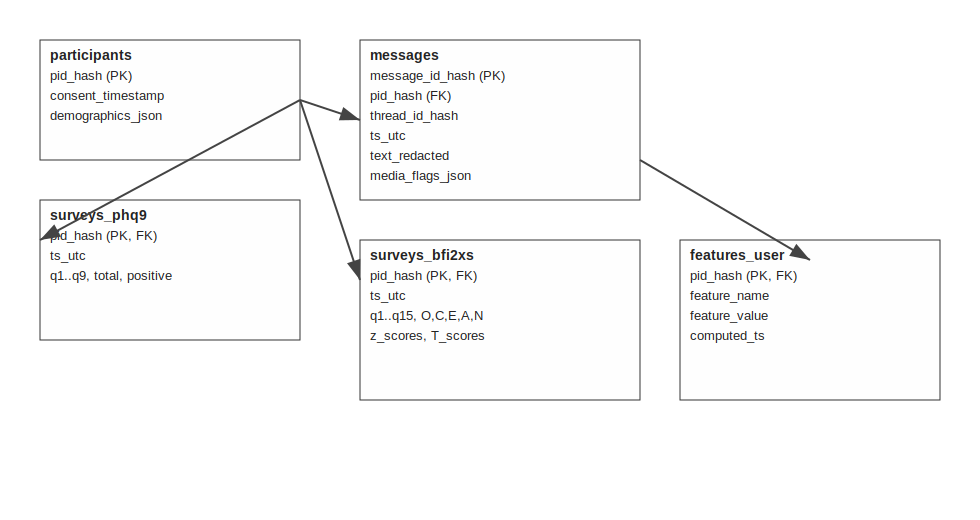
\includegraphics[width=0.9\linewidth]{thesis/figures/schema.svg}
  \caption{Entity-relationship schema for storage and processing.}
  \label{fig:schema}
\end{figure}

\section{Data Flow and Processing Pipeline}
\label{sec:dataset-flow}
The end-to-end flow is depicted in Figure~\ref{fig:data-flow}: collection \(\to\) de-identification \(\to\) encrypted storage \(\to\) preprocessing \(\to\) feature extraction \(\to\) modeling \(\to\) evaluation. Each stage writes audit logs and immutable manifests (row counts, feature counts, hash digests) to support reproducibility and integrity checks.

\begin{figure}[t]
  \centering
  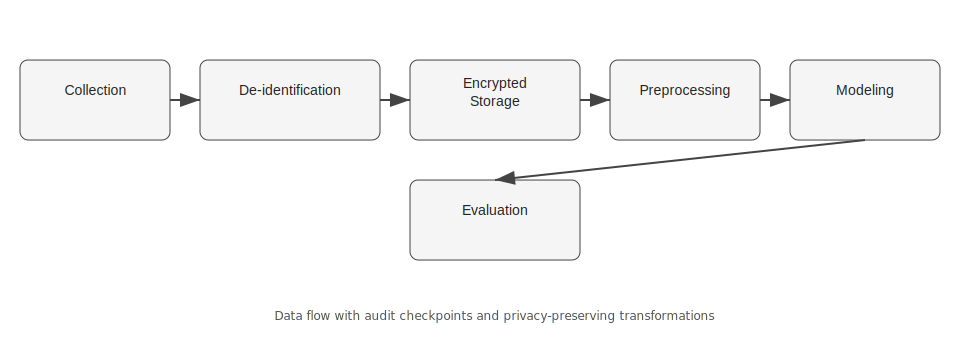
\includegraphics[width=0.95\linewidth]{thesis/figures/data_flow.svg}
  \caption{Data flow from collection to evaluation with privacy-preserving transformations and audit checkpoints.}
  \label{fig:data-flow}
\end{figure}

\section{Ethics, Privacy, and Risk Mitigation}
\label{sec:dataset-ethics}
\paragraph{IRB protocol summary.} The IRB reviewed and approved the protocol including recruitment, consent, data handling, and risk procedures. The protocol emphasizes data minimization, de-identification, and limited access. Participants may withdraw without penalty.

\paragraph{Confidentiality and security.} Encryption in transit (TLS 1.3) and at rest (AES-256-GCM) is enforced. Access is limited to named personnel, requires MFA, and is time-bounded. Audit logs are retained. Data are stored in a compliant environment (e.g., ISO 27001).

\paragraph{Risk mitigation.} PHQ-9 item 9 (suicidality) responses \(>0\) trigger an immediate on-screen safety resource page with crisis hotline information and optional contact with study staff. No clinical diagnosis is provided. We do not attempt to detect crises from messages.

\paragraph{Third-party privacy.} Only participant-authored messages are retained. Peer identifiers are pseudonymized. We publish only aggregate statistics and privacy-safe paraphrased exemplars in error analysis (Section~\ref{sec:methods-error-analysis}).

\section{Tables}
\begin{table}[t]
\centering
\caption{PHQ-9 items, response options, and scoring rules. Binary label positive if total score \(\geq 10\).}
\label{tab:phq9-scoring}
\begin{tabular}{p{0.06\linewidth}p{0.74\linewidth}p{0.16\linewidth}}
\toprule
Item & Prompt (past two weeks) & Scoring \\
\midrule
1 & Little interest or pleasure in doing things & 0--3 \\
2 & Feeling down, depressed, or hopeless & 0--3 \\
3 & Trouble falling or staying asleep, or sleeping too much & 0--3 \\
4 & Feeling tired or having little energy & 0--3 \\
5 & Poor appetite or overeating & 0--3 \\
6 & Feeling bad about yourself — or that you are a failure or have let yourself or your family down & 0--3 \\
7 & Trouble concentrating on things, such as reading the newspaper or watching television & 0--3 \\
8 & Moving or speaking so slowly that other people could have noticed? Or the opposite — being so fidgety or restless that you have been moving around a lot more than usual & 0--3 \\
9 & Thoughts that you would be better off dead or of hurting yourself in some way & 0--3 \\
\midrule
Total & \(S_{\text{PHQ}} = \sum_{i=1}^{9} x_i\), range 0--27 & Positive if \(\geq 10\) \\
Missing & If one item missing, impute with rounded mean; if \(\geq 2\) missing, invalid & -- \\
\bottomrule
\end{tabular}
\end{table}


\begin{table}[t]
\centering
\caption{BFI-2-XS item-to-domain mapping and reverse-key flags. Items use a 1--5 Likert scale. Reverse-keyed items are transformed as \(z = 6 - x\). Domain score is the mean of three keyed items; z- and T-scores standardized across the sample.}
\label{tab:bfi2xs-scoring}
\begin{tabular}{p{0.08\linewidth}p{0.20\linewidth}p{0.12\linewidth}p{0.48\linewidth}}
\toprule
Item & Domain & Reverse (R) & Item stem (abbrev.) \\
\midrule
1 & Extraversion (E) &  & Is outgoing, sociable \\
2 & Agreeableness (A) & R & Is compassionate, has a soft heart (rev) \\
3 & Conscientiousness (C) &  & Is organized, likes order \\
4 & Neuroticism (N) &  & Is anxious, easily upset \\
5 & Openness (O) &  & Has a vivid imagination \\
6 & Extraversion (E) & R & Is reserved, quiet (rev) \\
7 & Agreeableness (A) &  & Is respectful, treats others with respect \\
8 & Conscientiousness (C) & R & Tends to be lazy (rev) \\
9 & Neuroticism (N) & R & Is emotionally stable, handles stress well (rev) \\
10 & Openness (O) & R & Has difficulty imagining things (rev) \\
11 & Extraversion (E) &  & Is full of energy \\
12 & Agreeableness (A) &  & Is considerate and kind to almost everyone \\
13 & Conscientiousness (C) &  & Is reliable, can be counted on \\
14 & Neuroticism (N) &  & Gets easily distracted, has trouble focusing \\
15 & Openness (O) &  & Is curious about many different things \\
\midrule
Scoring & Domain means &  & For domain d: key items, reverse R, mean to get s_d; z/T standardized across sample \\
Missing & Handling &  & If one item missing in domain, mean of remaining two; if \(\geq 2\) missing, domain set to missing \\
\bottomrule
\end{tabular}
\end{table}



